\section{Instruction Set Simulation}

\subsection{Introduction to Simulation}

\begin{frame}{Instruction Set Simulation}

What is Instruction Set Simulation? 

\begin{itemize}
\item<2-> Model a partial or complete computer system
\item<3-> Potentially add instrumentation or perform analysis
\item<4-> May be timing accurate
\end{itemize}

\only<2-5>{
\centering
\onslide<2->{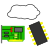
\includegraphics[width=0.25\textwidth]{figures/computers}}
\qquad
\onslide<3->{
\includegraphics[width=0.25\textwidth]{figures/instrumentation}}
\qquad
\onslide<4->{
\includegraphics[width=0.25\textwidth]{figures/stopwatch}}
}

\onslide<5->{
Note that this also covers associated technologies!
%e.g. binary instrumentation, virtualisation
}
\end{frame}

\begin{frame}[t]{Instruction Set Simulation}
\vspace{0pt}
\begin{minipage}{\textwidth}
	\vspace{0pt}
	Instruction Set Simulation is used in a wide variety of contexts:
	\begin{itemize}
		\item<2-> Design Space Exploration
%		\only<2>{
%			\begin{itemize}
%				\item Gem5
%				\item Multi2Sim
%			\end{itemize}
%		}
		\item<3-> Software Development 
%		\only<3>{
%			\begin{itemize}
%				\item QEMU
%				\item Android Emulator
%			\end{itemize}
%		}
		\item<4-> Backwards Compatibility
%		\only<4>{
%			\begin{itemize}
%				\item Apple Rosetta
%				\item Nintendo NES Classic
%				\item XBox One
%			\end{itemize}	
%		}
	\end{itemize}
\end{minipage}

\bigskip

\only<2>{
	\begin{figure}
		
\includegraphics[height=80pt]{figures/gem5-logo}
	\end{figure}
}
\only<3>{
	\begin{figure}
		
\includegraphics[height=80pt]{figures/android-logo-large}
	\end{figure}
}
\only<4>{
	\begin{figure}
		\centering
		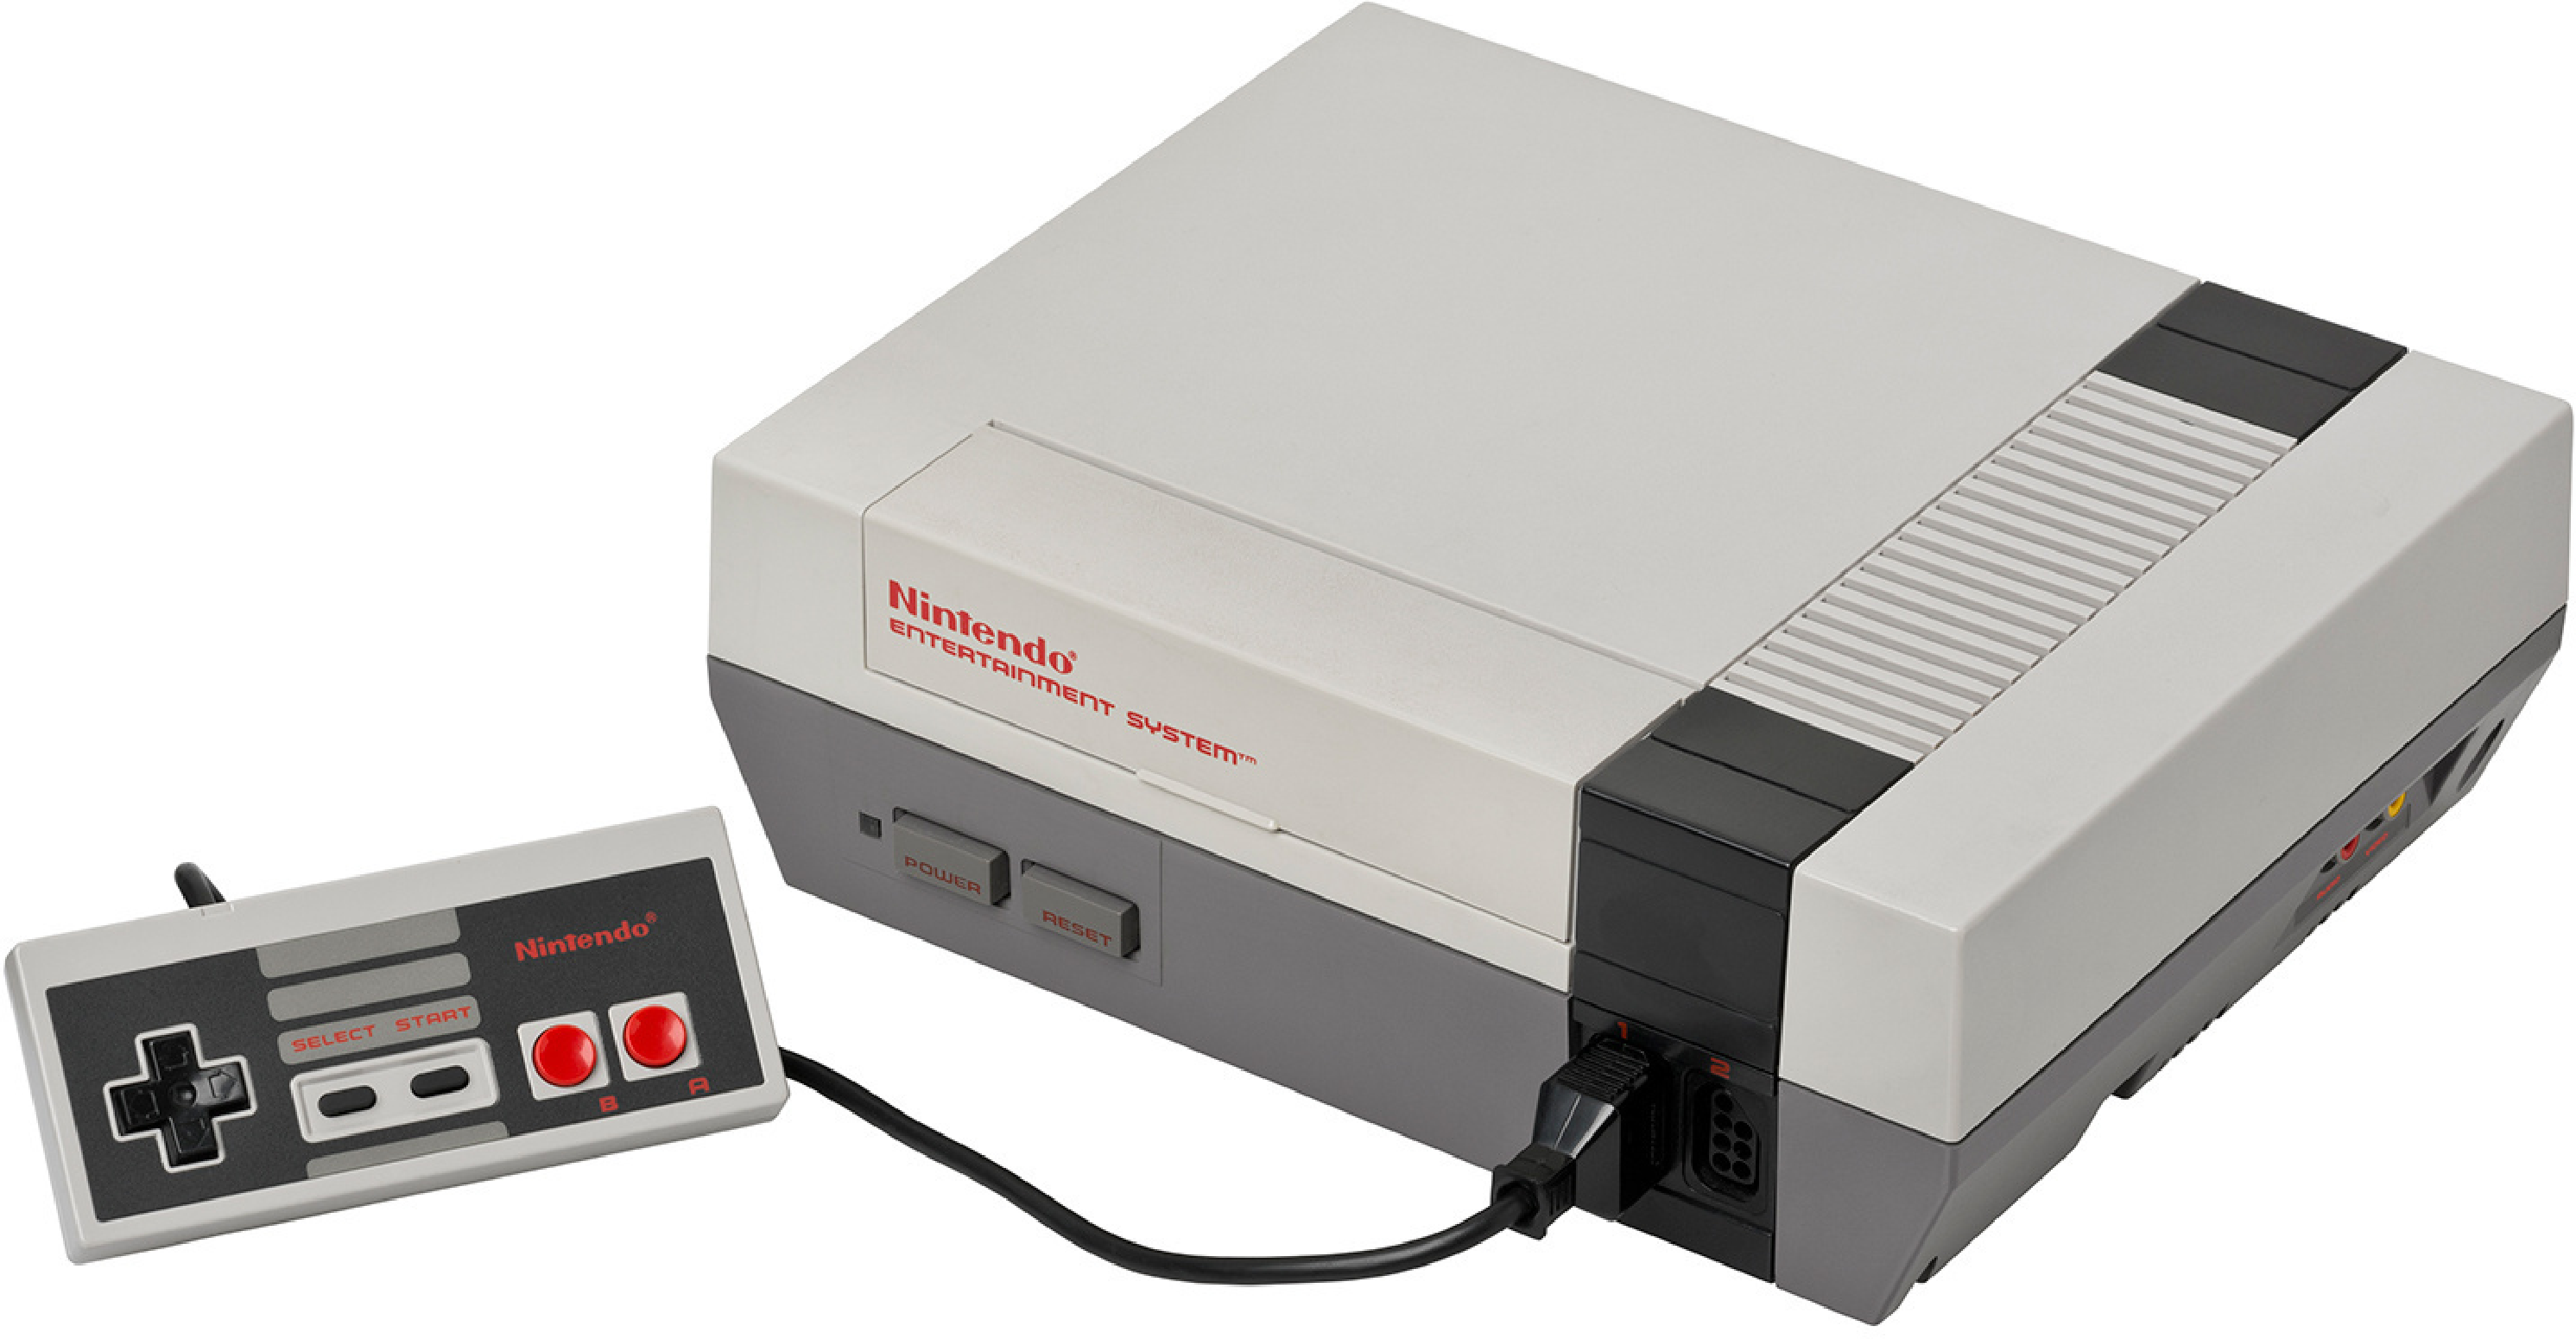
\includegraphics[height=70pt]{figures/nintendo-classic}
		\qquad
		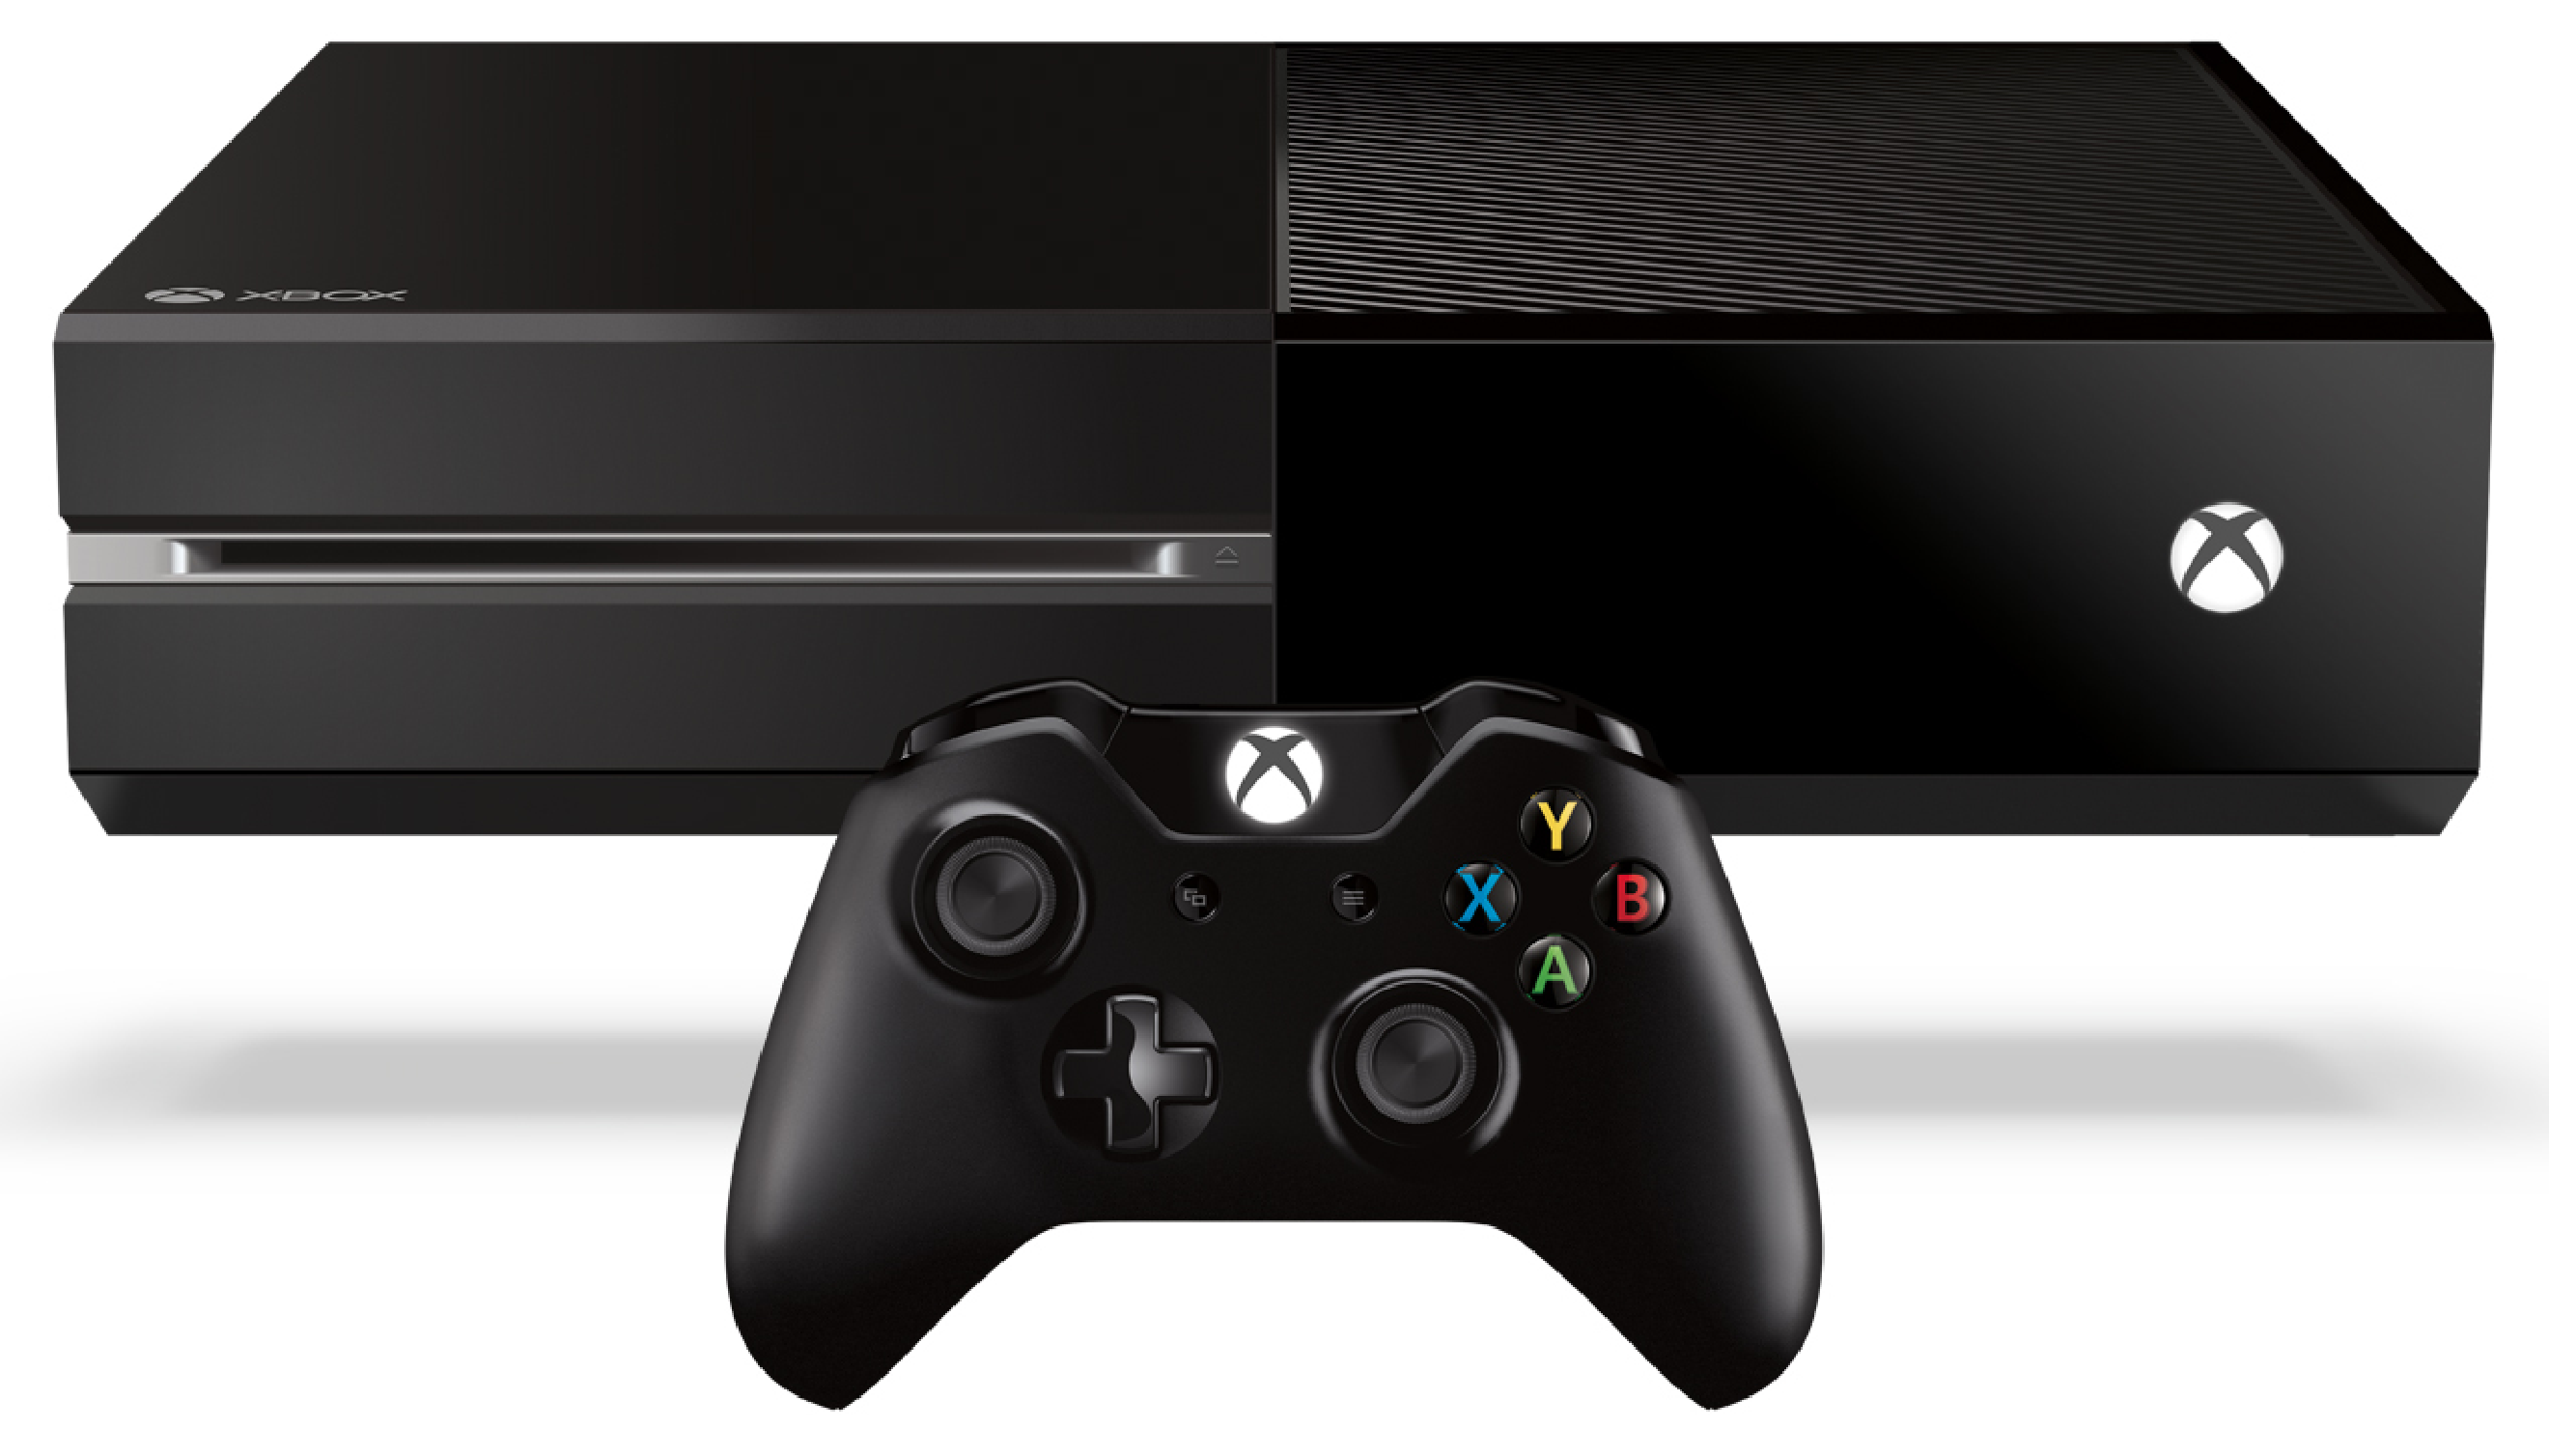
\includegraphics[height=70pt]{figures/xbox-one}
	\end{figure}
}

\end{frame}

\begin{frame}{Simulation Technologies}

Broadly, there are two software-based simulation technologies:

\bigskip

\centering
\begin{tabular}{l l l}
Technology & Slowdown & Complexity \\
\hline
Interpretation & 1000x & Low \\
\alert<2->{Binary Translation} & \alert<2->{10x} & \alert<2->{High} \\

\end{tabular}

\bigskip

\onslide<3>{Can we get the \alert{speed} of BT without the \alert{complexity}?}

\end{frame}

\begin{frame}[fragile]{Example QEMU Instruction}
\begin{lstlisting}[language=C]
target_long imm = sextract64(inst, 20,12);
int rs1 = extract32(inst, 15, 5);
int rd  = extract32(inst, 7, 5);
TCGv source1 = tcg_temp_new();
gen_get_gpr(source1, rs1);
tcg_gen_addi_tl(source1, source1, imm);
gen_set_gpr(rd, source1);
tcg_temp_free(source1);
\end{lstlisting}
\end{frame}

\subsection{Architecture Description Languages}

\begin{frame}
\frametitle{Architecture Description Languages}

ADLs are useful tools for systems development. They let us:
\begin{itemize}
	\item<2-> ...describe systems at different levels of abstraction
	\item<3-> ...use new technologies without rewriting all of our tools
	\item<4-> ...separate the behaviour of tools from their implementation
\end{itemize}

\bigskip

\centering
\onslide<2->{
	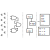
\includegraphics[width=0.25\textwidth]{figures/adl-levels-small}\qquad
}
\onslide<3->{
	
\includegraphics[width=0.25\textwidth]{figures/tool-portability}\qquad
}
\onslide<4->{
	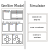
\includegraphics[width=0.25\textwidth]{figures/implementation-separation}
}

\end{frame}

\begin{frame}[fragile]{QEMU/ADL Comparison}
    \begin{minipage}{0.48\textwidth}
        \begin{lstlisting}[language=C,basicstyle=\tt\tiny,frame=single]
target_long imm = sextract64(inst, 20,12);
int rs1 = extract32(inst, 15, 5);
int rd  = extract32(inst, 7, 5);
TCGv source1 = tcg_temp_new();
gen_get_gpr(source1, rs1);
tcg_gen_addi_tl(source1, source1, imm);
gen_set_gpr(rd, source1);
tcg_temp_free(source1);
        \end{lstlisting}
        
    \end{minipage} %
    \quad %
    \begin{minipage}{0.47\textwidth}
\begin{lstlisting}[basicstyle=\tt\tiny,frame=single]
sint32 imm = inst.imm;
imm <<= 20;
imm >>= 20;

sint32 rs = read_register_bank(inst.rs1);

rs += imm;

write_register_bank(GPR, inst.rd, rs);
    \end{lstlisting}
    \end{minipage}
\end{frame}

\begin{frame}
\centering
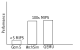
\includegraphics{figures/comparison-chart}
\end{frame}

\begin{frame}
\frametitle{Architecture Description Languages}

We consider ADLs mostly in the context of simulation
\begin{itemize}
	\item Low level ADLs are more suited to detailed simulation
	\item More abstract ADLs are better suited to fast simulation
\end{itemize}

\centering
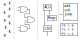
\includegraphics[width=0.8\textwidth]{figures/adl-levels}

\end{frame}
